\documentclass[brudnopis]{xmgr}
% Jeśli nowe rozdziały mają się zaczynać na stronach
% nieparzystych:
%\documentclass[openright]{xmgr}

%\defaultfontfeatures{Scale=MatchLowercase}
%\setmainfont[Numbers=OldStyle,Ligatures=TeX]{Minion Pro}
%\setsansfont[Numbers=OldStyle,Ligatures=TeX]{Myriad Pro}
% for fontspec version < 2.0
\setmainfont[Numbers=OldStyle,Mapping=tex-text]{Minion Pro}
\setsansfont[Numbers=OldStyle,Mapping=tex-text]{Myriad Pro}
%\setmonofont[Scale=0.75]{Monaco}
% Opcjonalnie identyfikator dokumentu

\author   {Marcin Dawidowski}
\nralbumu {231010}
\email    {marcin.dawidowskipl@gmail.com}

\title    {Let’s Bid It – portal aukcyjny}
\date     {2017}
\miejsce  {Gdańsk}

\opiekun  {dr Włodzimierz Bzyl}

% dodatkowe polecenia
%\renewcommand{\filename}[1]{\texttt{#1}}
%\definecolor{stress}{cmyk}{0,1,0.13,0} % RubineRed
%\definecolor{topic}{cmyk}{0.98,0.13,0,0.43} % MidnightBlue

\begin{document}

% streszczenie
\begin{abstract}
  W pracy przedstawiono rozwojową wersję aplikacji webowej „Let's Bid It” służącą do tworzenia i publikowania aukcji oraz ogłoszeń.

  W aplikacji zaimplementowano tworzenie kont użytkowników i administratorów, a także zarządzanie nimi. Ponadto dodany został mechanizm reCAPTCHA, który sprawdza rejestrującego się aktualnie użytkownika.  Wdrożona również została kategoryzacja aukcji, ich wyszukiwanie, a także dodawanie i usuwanie z obserwowanych . Możliwa jest również licytacja aukcji po zalogowaniu się na konto użytkownika. Dodatkowo zaimplementowane zostały kategorie, które można tworzyć w hierarchii.

  Zaprojektowano widok strony głównej, na której wyświetlane są główne kategorie, a także najnowsze aukcje znajdujące się w portalu. Ponadto po zalogowaniu na konto użytkownika, na stronie głównej widoczne są aktualnie obserwowane przez niego aukcje. Utworzone również zostały widoki aukcji, kategorii, obserwowanych, a także statystyki. Ponadto zaimplementowano panel administracyjny i panel użytkownika, które są widoczne po zalogowaniu się na konkretny typ konta. Ponadto wykonane zostały górny oraz dolny pasek nawigacyjny, które wyświetlają różne odnośniki zależnie od typu użytkownika.

  Do tworzenia aplikacji użyty został język Ruby z wykorzystaniem frameworka Rails, a także Twitter Bootstrap, Plataformatec Devise, reCAPTCHA, CKEditor, jQuery Turbolinks, Chartkick, ActsAsTree oraz Font-Awesome.

\mbox{Projekt wdrożony został na platformie\, \\\texttt{heroku.com} i jest dostępny pod adresem:} \\\texttt{\url{https://ror-aukcja.herokuapp.com/}}\footnote{W celu zalogowania się na konto użytkownika należy kliknąć przycisk "Logowanie" w górnym pasku nawigacyjnym, natomiast aby zalogować się na konto administratora należy użyć linku "Administracja" w stopce strony. Do logowania należy użyć następujących danych: konto administratora: \texttt{admin@admin.pl}, konto użytkownika: \texttt{user@user.pl}, hasło do obu kont to \texttt{admin1}.}

Kod źródłowy aplikacji dostępny jest natomiast na platformie Github pod adresem: \\\texttt{\url{https://github.com/mdawidowski/praca_licencjacka}}


\end{abstract}

% słowa kluczowe
\keywords{ruby on rails, gem, heroku, auction, online shopping, bid, recaptcha}

% tytuł i spis treści
\maketitle

% wstęp
\introduction

Chęć stworzenia czegoś od podstaw oraz własne doświadczenie w korzystaniu z portali aukcyjnych sprawiło, że dla mnie jako programisty stworzenie takiej aplikacji, byłoby niezwykle satysfakcjonujące i pozwoliłoby rozwinąć umiejętności. Ponadto stworzenie takiego portalu może ułatwić mi w przyszłości implementacje różnego rodzaju sklepów internetowych i innych serwisów związanych z handlem przez Internet.

Mając więc gotowy pomysł na projekt pozostało mi jedynie wybrać odpowiednią technologię, która pomoże mi go zrealizować. W trakcie studiów poznałem kilka różnych języków programowania i frameworków, które sprawdziłyby się w tego typu projekcie. Po rozważeniu wszystkich za i przeciw, mój wybór padł na język Ruby, wspierany przez framework Rails, który udało mi się poznać już wcześniej. Największą zaletą wybranej przeze mnie technologi jest przede wszystkim fakt, iż Ruby on Rails posiada szeroką gamę dostępnych rozwiązań w postaci gemów, które w dużym stopniu ułatwiają pracę nad projektem. Kolejną kwestią jest fakt, że technologia  ta wykorzystuje architekturę MVC, co znacznie ułatwia pracę. Poza tym Ruby on Rails świetnie współpracuje z platformami takimi jak Heroku, czy DigitalOcean.

Aplikacja Let's Bid It jest wersją rozwojową portalu aukcyjnego, dlatego też nie posiada jeszcze wszystkich funkcjonalności, które pozwoliłyby w pełni wykorzystać potencjał serwisu.

Spośród rzeczy, które udało się zrealizować, mogę wyróżnić przede wszystkim obsługę aukcji. Ponadto zaimplementowano ich kategoryzację przy pomocy gemu Act as tree. Kolejną rzeczą jest wdrożenie zaawansowanego edytora tekstowego CKEditor, dzięki któremu dodając aukcję, użytkownik może swobodnie manipulować jej opisem. Dodatkowo zaimplementowałem zabezpieczenie reCAPTCHA przy logowaniu i rejestracji, a także statystyki strony, które dostępne są dla administratorów. Ważnym elementem Let's Bid It jest również grafika dołączana do każdej aukcji. W związku z tym, że aplikacja znajduje się na platformie Heroku, głównym problemem było przetrzymywanie plików graficznych, które na Heroku usuwane są automatycznie. Rozwiązaniem tego problemu okazało się skorzystanie z serwisu Cloudinary, który pozwala bezpłatnie przechowywać pliki w chmurze, a co najważniejsze, możliwe jest skonfigurowanie go tak, by współpracował z aplikacją napisaną w Ruby on Rails, w czym pomocny okazał się gem cloudinary.

Najważniejszą rzeczą, której nie udało się zrealizować jest wdrożenie systemu mającego na celu symulacje płatności internetowych, a także zaawansowana wyszukiwarka opierająca się na silniku Elasticsearch.


\chapter{Let's Bid It w praktyce}

\section{Porównanie z dostępnymi rozwiązaniami}

\subsection{Allegro}

Jest to największa, a także najpopularniejsza platforma transakcyjna on-line w Polsce, oferująca setki produktów w niezwykle konkurencyjnych cenach. Serwis udostępnia możliwość zakupu natychmiastowego, licytacji, a także wystawiania ogłoszeń. Typ danej aukcji, zależy tylko i wyłącznie od jej właściciela.

Jeśli chodzi o wystawianie aukcji, to proces wygląda podobnie do Let's Bid It. Tak jak w mojej aplikacji użytkownik może skorzystać z zaawansowanego edytora tekstowego, dodaje zdjęcia i przyporządkowuje ją do konkretnej kategorii. Główną różnicą jest fakt, że Allegro pozwala na wystawienie przedmiotu z użyciem opcji „Kup Teraz”, czego Let's Bid It nie ma.

\subsection{OLX}

Serwis ten jest jednym z najpopularniejszych portali ogłoszeniowych na świecie. Użytkownicy
mogą udostępniać lokalne ogłoszenia dotyczące sprzedaży oraz usług.

Główną różnicą pomiędzy OLX, a Let's Bid It jest fakt,
że wymieniony wyżej portal nie udostępnia funkcji licytacji towaru, natomiast moja aplikacja posiada ją, a także tak jak OLX daje użytkownikowi prawo wystawienia towaru, czy też usługi jako zwykłe ogłoszenie. Ponadto stworzony przeze mnie portal aukcyjny, dzięki zaawansowanemu edytorowi tekstowemu pozwala stworzyć użytkownikom dużo bardziej oryginalne opisy, co nie jest możliwe przy korzystaniu z wyżej wymienionego portalu.

\section{Możliwości zastosowania praktycznego}
Głównym założeniem serwisu Let's Bid It jest przede wszystkim portal aukcyjny i jest to główna możliwość zastosowania napisanej przeze mnie aplikacji w praktyce. Poza tym portal ten użyty może zostać również do innych celów:

\begin{itemize}

\item Portal ogłoszeniowy – jest jedną z możliwości wykorzystania Let's Bid It. Potrzeby takiej aplikacji zaspokajają praktycznie wszystkie wdrożone w mojej aplikacji funkcjonalności, takie jak kategoryzacja, a także prosta obsługa dodanych ogłoszeń. Ponadto użytkownik takiego  serwisu będzie miał do dyspozycji bardzo prosty interfejs ułatwiający poruszanie się po stronie, a także zaawansowany edytor, który pozwoli na to, by jego ogłoszenie wyglądało wyjątkowo.

\item Sklep internetowy – jest to kolejna możliwa opcją zastosowania mojej aplikacji w praktyce, co można osiągnąć przy niedużym nakładzie pracy. Tak jak przy portalu ogłoszeniowym, dostępne są przede wszystkim kategoryzacja, a także obsługa dodawanych aukcji oraz zaawansowane narzędzia do zarządzania wyglądem aukcji.

\end{itemize}

\chapter{Projekt i analiza}

\section{Diagram ERD}

\begin{figure}[!tbh]
\centering
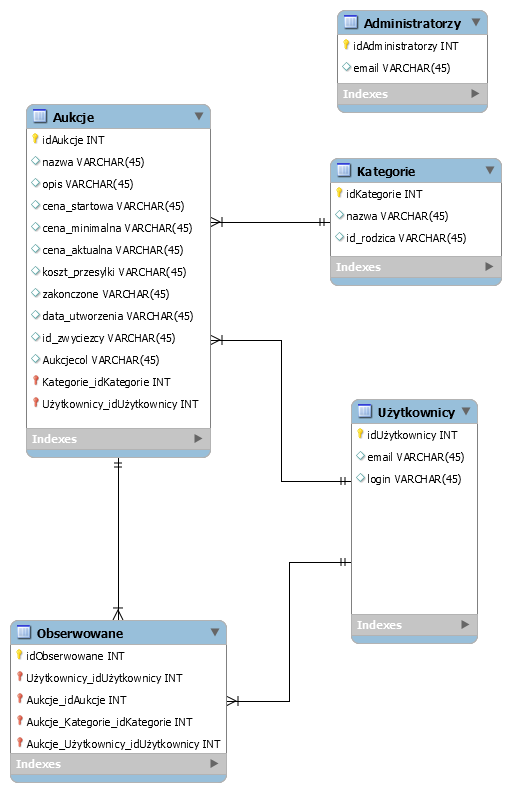
\includegraphics[scale=0.4]{fig/erd}
\caption{Diagram związków encji\label{RYS.1}}
\source{Opracowanie własne za pomocą MySQL Workbench }
\end{figure}

\newpage

\section{Aktorzy i przypadki użycia}
\begin{figure}[!tbh]
\centering
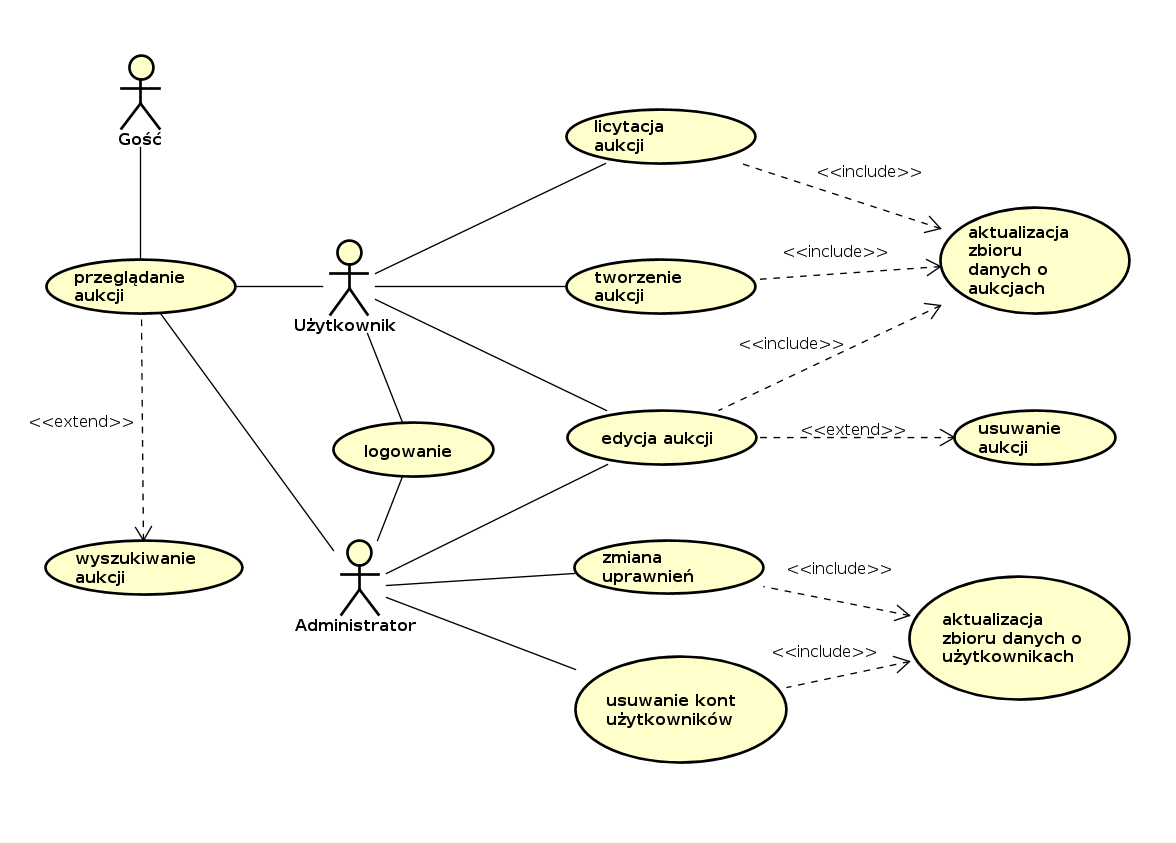
\includegraphics[width=\linewidth]{fig/ucdiagram}
\caption{Diagram Przypadków Użycia.}
\source{Opracowanie własne za pomocą programu Astah \cite{astah}.}
\end{figure}

\newpage

\section{Diagram przepływu danych}
\begin{figure}[!tbh]
\centering
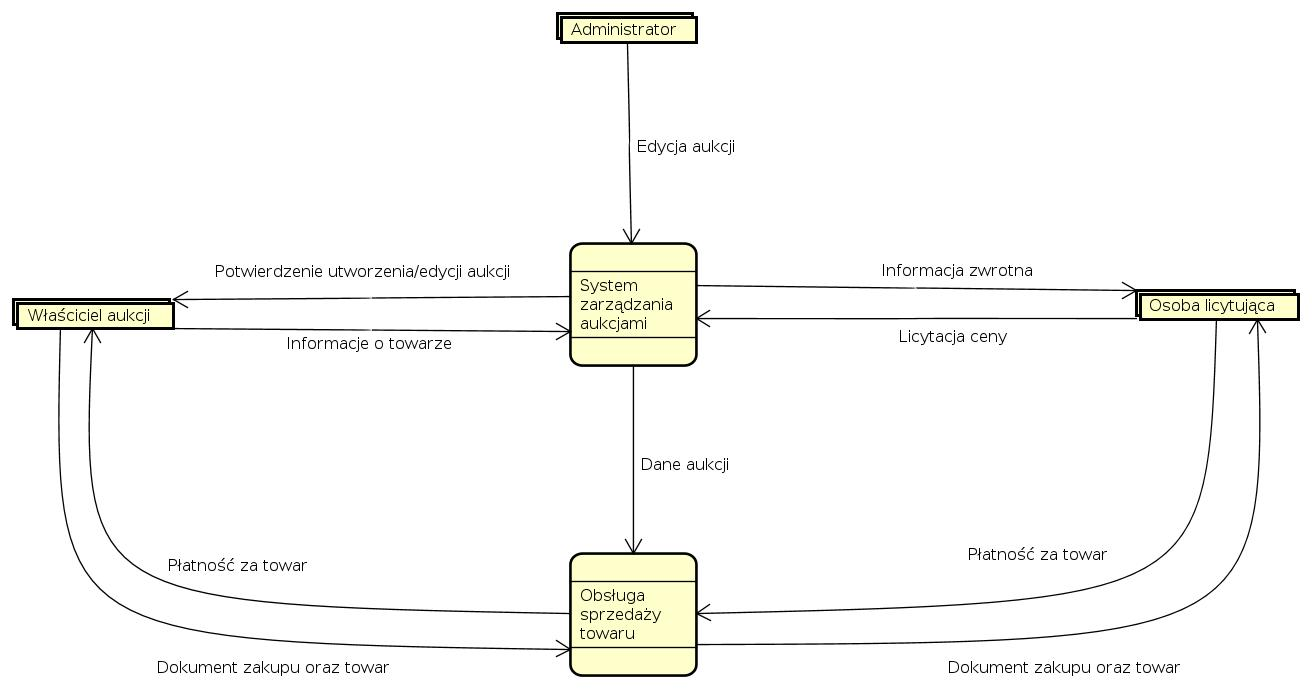
\includegraphics[width=\linewidth]{fig/DFD}
\caption{Diagram Przepływu Danych.}
\source{Opracowanie własne za pomocą programu Astah \cite{astah}.}
\end{figure}

\chapter{Implementacja}
W celu stworzenia aplikacji, która ma w odpowiedni sposób realizować postawione przed nią
założenia, potrzebne są odpowiednio dobrane technologie oraz narzędzia, dzięki którym uda się
spełnić postawione przed nią wymagania. Dobór odpowiedniej technologii, a także frameworków
jest kluczowy do skutecznej implementacji aplikacji.

\section{Ruby on Rails}
Do stworzenia projektu wykorzystana została technologia Ruby on Rails bazująca na języku Ruby.
W aplikacji wykorzystano Ruby w wersji 2.3, a także framework Rails w wersji 5.0.1. Całość stworzona
została przy pomocy architektury MVC (ang. Model-View-Controller).

\section{Twitter Bootstrap}
Widoki utworzone zostały przy pomocy frameworka Twitter Bootstrap, który pozwala na proste tworzenie
graficznego interfejsu stron internetowych z wykorzystaniem gotowych rozwiązań bazujących na językach
HTML i CSS. Główną zaletą tego frameworka jest responsywność, czyli zapewnienie poprawnego wyświetlania
stron WWW na różnych urządzeniach.

Aby wdrożyć Twitter Bootstrap do aplikacji wymagane jest jedynie dopisanie poniższej linijki do pliku Gemfile
re
\section{Devise}

Budując portal aukcyjny koniecznym wymogiem jest przede wszystkim obsługa użytkowników i administratorów aplikacji. W tym celu wdrożony został gem Devise, który w znacznym stopniu ułatwia autentykację na stronie. Dzięki zastosowaniu powyższego gemu otrzymujemy niemalże gotowe widoki, kontroler oraz model, co pozwala na bezproblemowe zarządzanie użytkownikami.

\section{Pozostałe rozwiązania użyte przy realizacji projektu}

\subsection{Cloudinary}

Serwis pozwalający na przechowywanie danych w chmurze. Dzięki połączeniu go z aplikacją możliwe było bezproblemowe przechowywanie grafik dołączanych przez użytkowników do aukcji i rozwiązanie problematycznego przechowywania tych plików na serwerze Heroku.

\subsection{ActsAsTree}

Gem ułatwiający tworzenie kategorii w postaci drzewa. Poprawia w sposób zdecydowany nawigację
po stronie, a także sprawia, że dane są uporządkowane. Sama implementacja przebiega w środowisku
technologii Ruby on Rails, więc nie wymaga bezpośredniej instalacji.

\subsection{reCAPTCHA}

Zabezpieczenie dzięki któremu możliwość wysyłania danych będą mieli jedynie sprawdzeni użytkownicy.

\begin{figure}[!tbh]
\centering
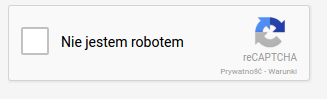
\includegraphics[scale=0.8]{fig/captcha}
\caption{Pole weryfikacyjne reCAPTHA.}
\source{Opracowanie własne.}
\end{figure}


\subsection{Chartkick}

Gem pozwalający na tworzenie i wyświetlanie różnego rodzaju wykresów na podstawie danych zawartych w aplikacji.

\begin{figure}[!tbh]
\centering
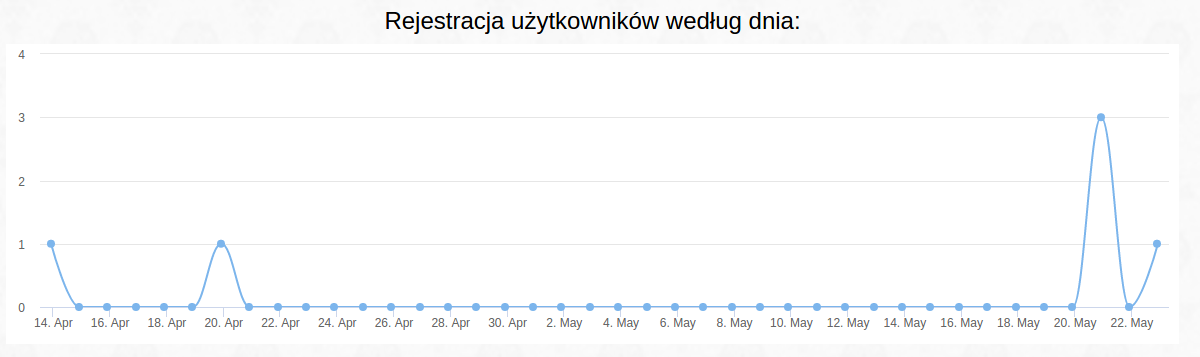
\includegraphics[width=\linewidth]{fig/chart}
\caption{Wykres utworzony przy pomocy gemu Chartkick.}
\source{Opracowanie własne.}
\end{figure}


\subsection{Font-Awesome}

Rozszerzenie dzięki któremu możliwe jest na umieszczenie w aplikacji skalowalnych ikon, co znacznym stopniu poprawia czytelność o raz wygląd strony.

\begin{figure}[!tbh]
\centering

\includegraphics[scale=0.5]{fig/icon}
\caption{Przykładowa ikona uzyskana dzięki gemowi Font-Awesome.}
\source{Opracowanie własne.}
\end{figure}


\subsection{CKEditor}

Wizualny edytor tekstowy języka HTML, który umożliwia użytkownikowi na wybranie między innymi konkretnej
czcionki, jej rozmiaru, koloru liter, czy też ich stylu. Poza tym użytkownik może również ustawić wyrównanie tekstu,
a także możliwe jest wstawienie listy, tabeli, odnośników, a także obrazów.

\begin{figure}[!tbh]
\centering
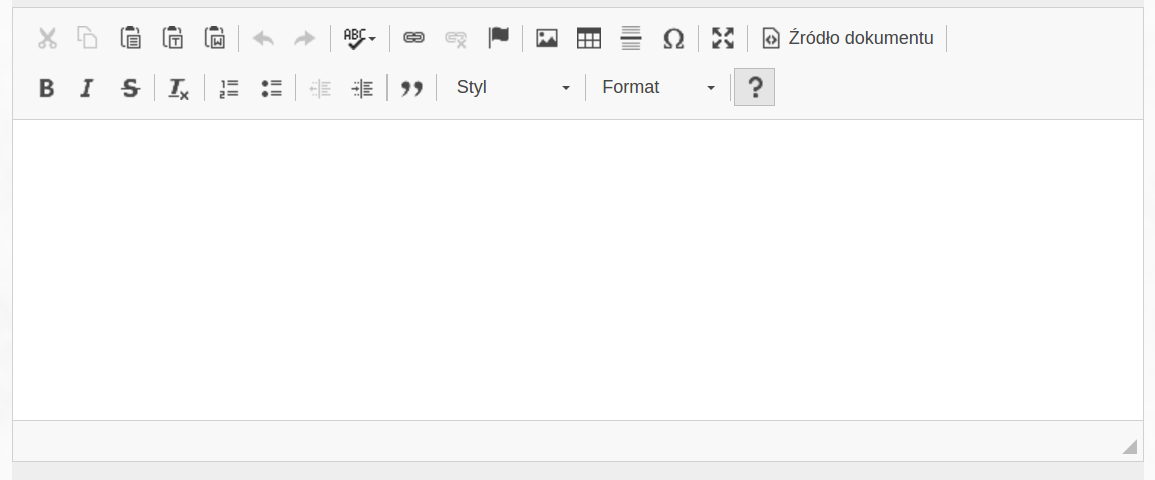
\includegraphics[width=\linewidth]{fig/ckeditor}
\caption{Zaawansowany edytor tekstu CKEditor.}
\source{Opracowanie własne.}
\end{figure}

\newpage

\section{Struktura aplikacji}

\subsection{Strona główna}

Strona główna aplikacji zaprojektowana została tak, aby w prosty sposób udostępniać wszystkie funkcjonalności aplikacji. Głównymi elementami strony głównej jest panel z wszystkimi nazwami kategorii nadrzędnych, a także miniatury wraz z tytułami losowo wybranych aukcji z całego ich zbioru. Ponadto po zalogowaniu na konto użytkownika, na stronie głównej informacje o aukcjach, które dany użytkownik dodał do obserwowanych.

\subsection{Aukcje}

Głównym elementem Let's Bid It są aukcje. Każda z nich posiada atrybuty takie jak:
\begin{itemize}

\item identyfikator autora aukcji
\item kategorię, do której należy
\item nazwę
\item szczegółowy opis
\item cenę początkową
\item cenę minimalną
\item koszt przesyłki
\item informację o tym, czy aukcja publikowana jest jako ogłoszenie
\item zdjęcie, które będzie publikowane jako główne.

\end{itemize}

Widok aukcji składa się z czterech stron, które różnią się ze względu na dostęp i wyświetlane na niej dane.

Pierwszym elementem jest strona index dostępna tylko dla zalogowanych użytkowników. Wyświetlane na niej są wszystkie aukcje, które utworzył aktualnie zalogowany użytkownik. Aukcje wyświetlane są w tabeli według identyfikatorów, zaś każdej aukcji przypisane są akcje pokaż, edytuj oraz usuń. W górze strony wyświetlany jest również odnośnik do utworzenia nowych aukcji przez aktualnie zalogowanego użytkownika.

Następnymi elementami aukcji są strony, które umożliwiają użytkownikom dodawanie oraz edytowanie aukcji. Są to dwa oddzielnie funkcjonujące elementy, jednak łączy je wspólny formularz wypełniany przy tworzeniu/edycji aukcji. Formularz ten zawiera wszystkie atrybuty aukcji, które zostały wymienione powyżej.

Najważniejszym elementem aukcji jest strona, na której każda z nich, jest wyświetlana wraz z wszystkimi informacjami, które zostały zawarte przy jej tworzeniu. Strona oraz wszystkie informacje na temat aukcji jest widoczna dla każdego, jednak niektóre jej funkcjonalności widoczne są jedynie dla zalogowanych użytkowników. Elementami, które widoczne są po zalogowaniu, to przycisk dodający aukcję do obserwowanych, a także panel, za pomocą którego możliwe jest licytowanie aukcji. Sam panel zabezpieczony został w taki sposób, aby niemożliwe było dodanie oferty niższej, lub takiej samej jak cena aktualna.

\subsection{Kategorie}

Uporządkowanie aukcji niemożliwe byłoby bez ich kategoryzacji, dlatego też koniecznym wydawało się wdrożenie kategorii, przy czym niezwykle pomocny był gem ActsAsTree.

Tak jak aukcje, kategorie składają się ze stron, które służą do ich dodawania, wyświetlania oraz edycji. Cechą różniącą kategorie i aukcje jest fakt, że strony oznaczone jako index, new oraz edit widoczne są tylko dla osób zalogowanych na konto administratora.

Ogólnodostępnym elementem kategorii jest widok udostępniający dane o konkretnej kategorii. Na stronie tej widoczne są wszystkie podkategorie danej kategorii, a także aukcję, które do niej należą.

\subsection{Obserwowane}

Dodanie aukcji do obserwowanych, jest jedną z funkcjonalności, która umożliwia łatwiejsze ich odnalezienie.

Widok opiera się na prostej tabeli, która wyświetla podstawowe dane na temat aukcji, które zostały dodane do obserwowanych. Rekordy tabeli wyposażone zostały również w przycisk, dzięki któremu możliwe jest usunięcie elementu z obserwowanych. W celu dodania aukcji do obserwowanych użytkownik musi odwiedzić stronę aukcji i kliknąć przycisk "Dodaj do obserwowanych". Jeśli jednak aukcja jest już obserwowana przez użytkownika, to na stronie wyświetlony zostanie przycisk "Przestań obserwować".

\subsection{Nawigacja}

Nawigacja na stronie umożliwiona została dzięki paskowi nawigacyjnemu, który umieszczony został na górze strony. Pasek ten w zależności od typu użytkownika wyświetla różne wartości.

Osoba odwiedzająca portal jako gość ujrzy na samej górze odnośnik do strony głównej, a także linki do rejestracji i logowania, które pozwolą na korzystanie z większej ilości funkcjonalności, które zostały wdrożone w Let's Bid It.

Zwykły użytkownik po zalogowaniu, poza odnośnikiem do strony głównej będzie miał również możliwość skorzystania z panelu użytkownika, edycji profilu, czy też po prostu z opcji wylogowania się z aktualnego konta.

Administrator strony, w odróżnieniu do użytkownika będzie mógł skorzystać z panelu administracyjnego, nie mając jednakowoż dostępu do panelu użytkownika. Pozostałe funkcje paska nawigacyjnego pozostaną takie same jak dostępne dla zalogowanego użytkownika.

\begin{figure}[!tbh]
\centering
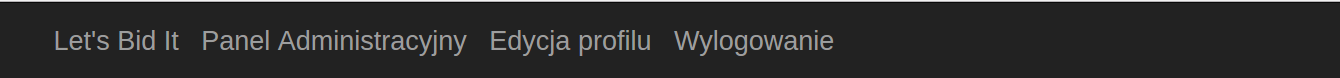
\includegraphics[width=\linewidth]{fig/pasek}
\caption{Przykładowy widok górnego paska nawigacyjnego.}
\source{Opracowanie własne.}
\end{figure}

Kolejnym elementem ułatwiającym poruszanie się po stronie jest dolny pasek nawigacyjny, popularnie zwany stopką. Zawiera on klauzulę Copyright, łącze do szerszych informacji na temat projektu, a także odnośnik przenoszący na stronę logowania dla administratora, który widoczny jest jedynie dla osób niezalogowanych. Po zalogowaniu na jakikolwiek typ konta odnośnik ten znika automatycznie.
\begin{figure}[!tbh]
\centering

\includegraphics[width=\linewidth]{fig/stopka}
\caption{Przykładowy widok dolnego paska nawigacyjnego.}
\source{Opracowanie własne.}
\end{figure}


% zakończenie
\summary
W trakcie pracy nad projektem udało mi się zrealizować praktycznie wszystkie jego założenia. Praca ta pozwoliła mi nabyć nowe doświadczenia, a także poszerzyć posiadane umiejętności. Podczas realizacji aplikacji udało mi się wykorzystać niemal wszystkie umiejętności, które nabyłem w trakcie odbywania studiów.

\begin{thebibliography}{9}

\bibitem{ror}
David A. Black.
\textit{Ruby. Przewodnik programisty wyd. II.}
HELION S.A. 2015.

\bibitem{ror}
John Elder.
\textit{Ruby on Rails - Tworzenie aplikacji WWW}
Codemy.com 2016.

\bibitem{bootstrap}
Michał Kortas.
\textit{Bootstrap. Praktyczne Projekty}
Helion 2016.

\bibitem{ror}
Oficjalna dokumentacja - Ruby on Rails (dostęp 1.03.2017)
\\\texttt{\url{https://github.com/rails/rails}}


\bibitem{devise}
Oficjalna dokumentacja - Gem Devise (dostęp 5.03.2017)
\\\texttt{\url{https://github.com/plataformatec/devise}}


\bibitem{actsastree}
Oficjalna dokumentacja - Gem ActsAsTree (dostęp 8.04.2017)
\\\texttt{\url{https://github.com/amerine/acts_as_tree}}


\bibitem{recaptcha}
Oficjalna dokumentacja - Gem reCAPTCHA  (dostęp 10.04.2017)
\\\texttt{\url{https://github.com/ambethia/recaptcha}}


\bibitem{ckeditor}
Oficjalna dokumentacja - Gem CKEditor for Rails (dostęp 10.04.2017)
\\\texttt{\url{https://github.com/galetahub/ckeditor}}


\bibitem{chartkick}
Oficjalna dokumentacja - Gem Chartkick (dostęp 28.04.2017)
\\\texttt{\url{https://github.com/ankane/chartkick}}


\bibitem{font-awesome}
Oficjalna dokumentacja - Gem Font-Awesome (dostęp 18.05.2017)
\\\texttt{\url{https://github.com/bokmann/font-awesome-rails}}


\bibitem{astah}
Oficjalna dokumentacja - Astah Professional (dostęp 10.04.2017)
\\\texttt{\url{http://astah.net/tutorials}}


\bibitem{mysql}
Oficjalna dokumentacja - MySQL Workbench (dostęp 10.04.2017)
\\\texttt{\url{https://dev.mysql.com/doc/workbench/en/}}

\end{thebibliography}

% załączniki (opcjonalnie):
\appendix
\chapter{Płyta CD zawierająca kod projektu}


\listoffigures


\oswiadczenie

\end{document}
